\section{Reading the map: a continuum, not biotypes}
\label{sec:strata}

The previous chapters delivered a \emph{map}: every one of the $9{,}013$ patients placed on nine validated
dimensions --- severity, two kinds of biology (metabolic, inflammatory), cognition, sleep, mania, suicidality,
developmental adversity, substance --- with diagnosis deliberately held out. This chapter asks the question the
whole ``precision psychiatry'' field chases: do patients fall into a handful of natural \emph{types} ---
biotypes --- that cut across the old diagnostic labels? The discipline here is to \emph{not assume the answer}.
The answer turns out to be \textbf{no}, and that negative reshapes what M2 \emph{is}: not a typology, but a
\textbf{coordinate system} for placing any patient, plus a \emph{reading guide} for interpreting positions.

\subsection{Ask whether types exist before imposing them}
\label{sub:continuum}
The classic error in clustering clinical data is to pick a number of clusters $K$ and then ``find'' $K$ groups
--- the algorithm always returns them, whether or not the data contain any. So before any clustering we run a
\textbf{structure-discovery gate} (Figure~\ref{fig:gateflow}): a battery of independent tests that each ask, in
a different language, \emph{is there cluster structure at all?} The decisive one is a \textbf{falsification
null} --- we compare the best partition of the real coordinates against the best partition of a single
structureless Gaussian blob with the same mean and covariance. If the real data separate no better than the
blob, there are no kinds to find.

\begin{figure}[h]\centering
\structuregateflow
\caption{Falsification-first. Before clustering, the best partition of the real coordinates is compared against a
structureless single-Gaussian null. On the FACE map the two are indistinguishable --- the verdict is a
\emph{continuum}, after which the cloud is described two honest ways: by its corners (a reading guide) and by
patient-to-patient similarity. The gate is the stratification analogue of the map chapter's ``the eligibility
map is itself a result.''}
\label{fig:gateflow}
\end{figure}

\begin{figure}[h]\centering
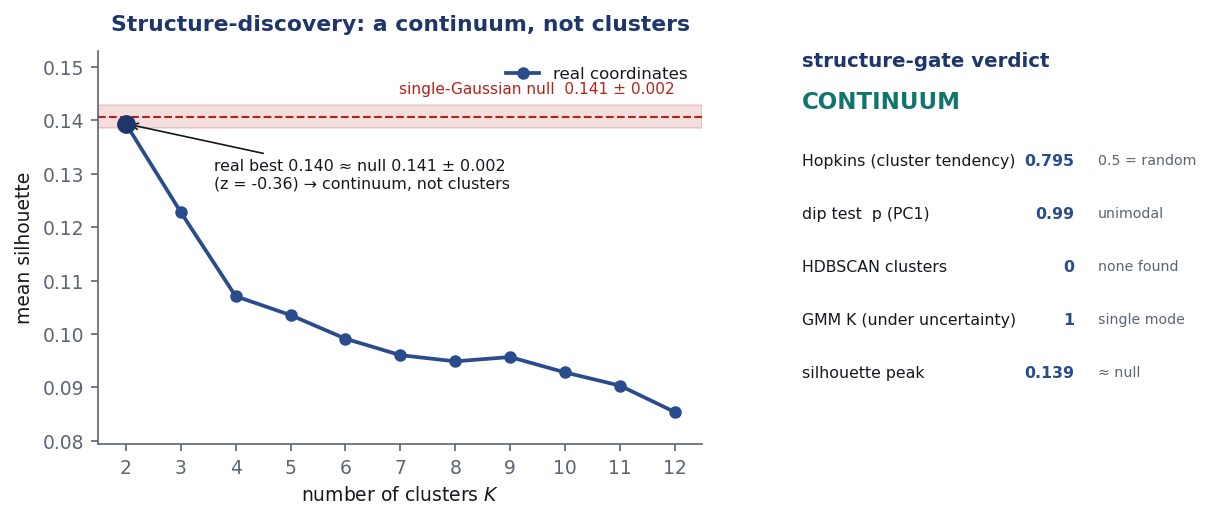
\includegraphics[width=0.92\linewidth]{figures/m2_structure.png}
\caption{The falsification null. \emph{Left:} silhouette by $K$ for the real coordinates --- the peak sits below
the $0.15$ separation floor and declines, so no $K$ yields separated groups. \emph{Right:} the best silhouette of
the real data ($0.140$) lands squarely inside the distribution of best silhouettes from a single-Gaussian blob
($0.141\pm0.002$, $z=-0.36$). The real cloud is statistically indistinguishable from a structureless continuum.}
\label{fig:structure}
\end{figure}

\begin{keyresult}[No evidence for discrete biotypes --- the space is a graded continuum]
The best partition of the real nine-dimensional cloud separates patients \emph{no better} than the best
partition of a structureless Gaussian blob (silhouette $0.140$ vs.\ $0.141\pm0.002$, $z=-0.36$). Four further
methods agree: the main axis is unimodal (dip $p\approx 0.99$), density clustering finds nothing (HDBSCAN: $0$
clusters), the topology is one connected component (Mapper), and once each patient's measurement uncertainty is
propagated the optimal number of mixture components collapses to $1$ in all $20$ posterior draws. There is no
hidden set of types. This lands where serious psychiatry has been heading (the dimensional RDoC/HiTOP view) and
says, with a test most ``biotype'' papers skip, that forcing a cluster count onto these data would manufacture
kinds the data do not contain.
\end{keyresult}

\subsection{What the map is: a coordinate system, not a set of types}
\label{sub:coordsystem}
If there are no types, what is the deliverable? It is the thing the map already gives: a patient's
\textbf{continuous position} on nine validated, transdiagnostic axes, with uncertainty. \emph{That} --- not any
set of boxes --- is the load-bearing object of M2, and it is what every downstream chapter actually consumes
(the temporal, prognosis and treatment models all run on the coordinates, never on a hard label). The corners
and regions introduced below are \textbf{reading lenses} on this continuum, not discoveries layered on top of it.

\begin{definitionbox}[Coordinate vs.\ type]
A \emph{type} answers ``which box is this patient in?'' --- and presumes the boxes exist. A \emph{coordinate}
answers ``where on the map is this patient, and how sure are we?'' --- which is well-defined whether or not boxes
exist. On a continuum only the second question is honest. So M2 ships coordinates, and the prognosis chapter
later confirms the choice empirically: \emph{no} hard partition adds predictive value beyond the continuous
position (\emph{operative $K=$ none}, \S\ref{sec:prognosis}).
\end{definitionbox}

\begin{figure}[h]\centering
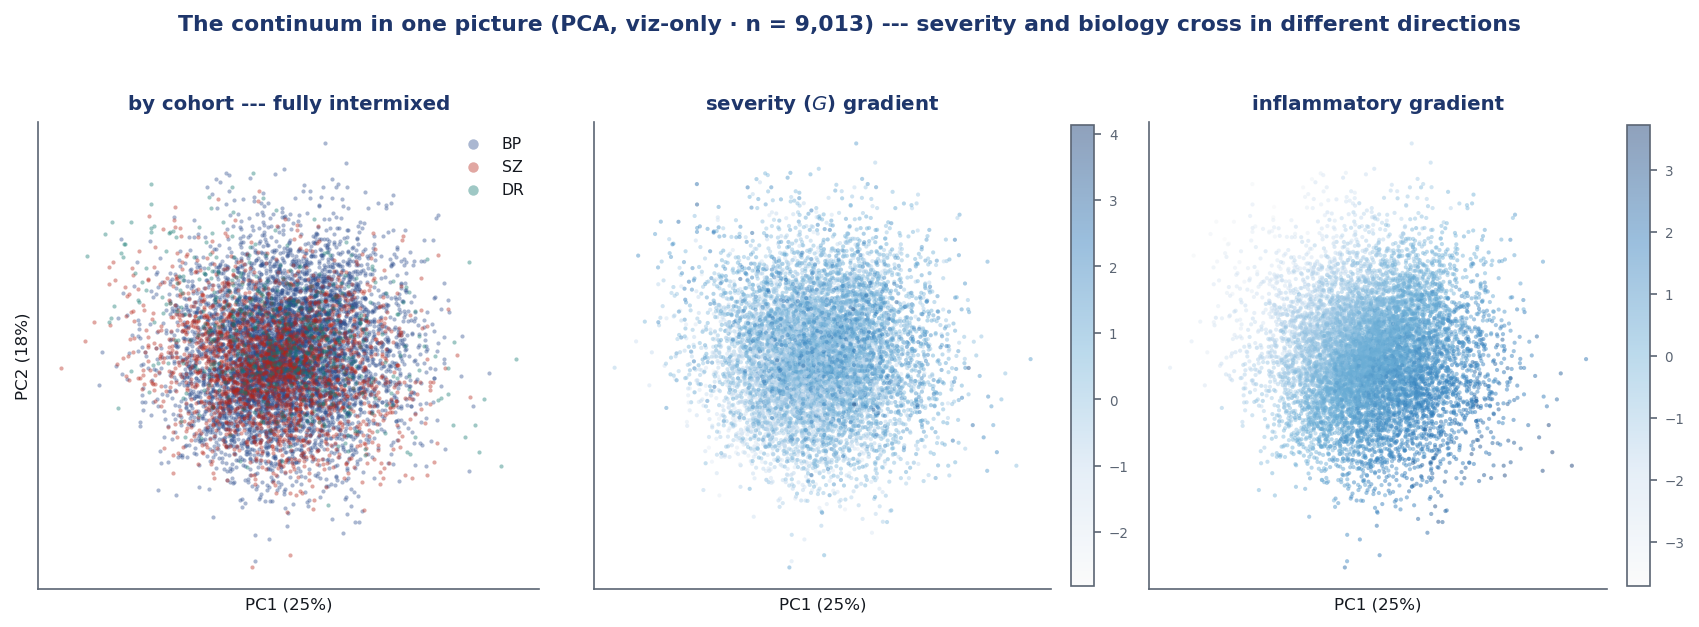
\includegraphics[width=\linewidth]{figures/m2_embedding.png}
\caption{The continuum in one picture (PCA, \emph{visualization-only} --- never a clustering input).
\emph{Left:} by cohort --- BP/SZ/DR fully intermixed, no diagnostic territories. \emph{Centre:} the severity
($G$) gradient. \emph{Right:} the inflammatory gradient --- crossing the cloud in a \emph{different} direction
from severity. One diffuse mass with crossing gradients, not a constellation of islands.}
\label{fig:embedding}
\end{figure}

\subsection{Reading the map (I): four corners and their representative patients}
\label{sub:reading}
A continuum has no clusters, but it still has a \emph{shape}, and the shape has \textbf{corners} --- extreme
phenotypes that the cloud stretches toward. Archetypal analysis recovers them: it finds a small set of extreme
profiles such that every patient is a convex \emph{blend} of them. Four corners are the stable resolution
(cross-seed Tucker congruence $0.98$; finer counts do not reproduce). Because a pure corner is an extreme almost
nobody sits exactly at, we report each corner three ways: its \textbf{pole} (the defining extreme), its
\textbf{typical representative} (the centroid of patients who lean toward it --- what a representative patient
looks like), and a real \textbf{exemplar} patient (the medoid). Plain clinical labels make them legible
(Figure~\ref{fig:readingguide}, Table~\ref{tab:reading}).

\begin{figure}[h]\centering
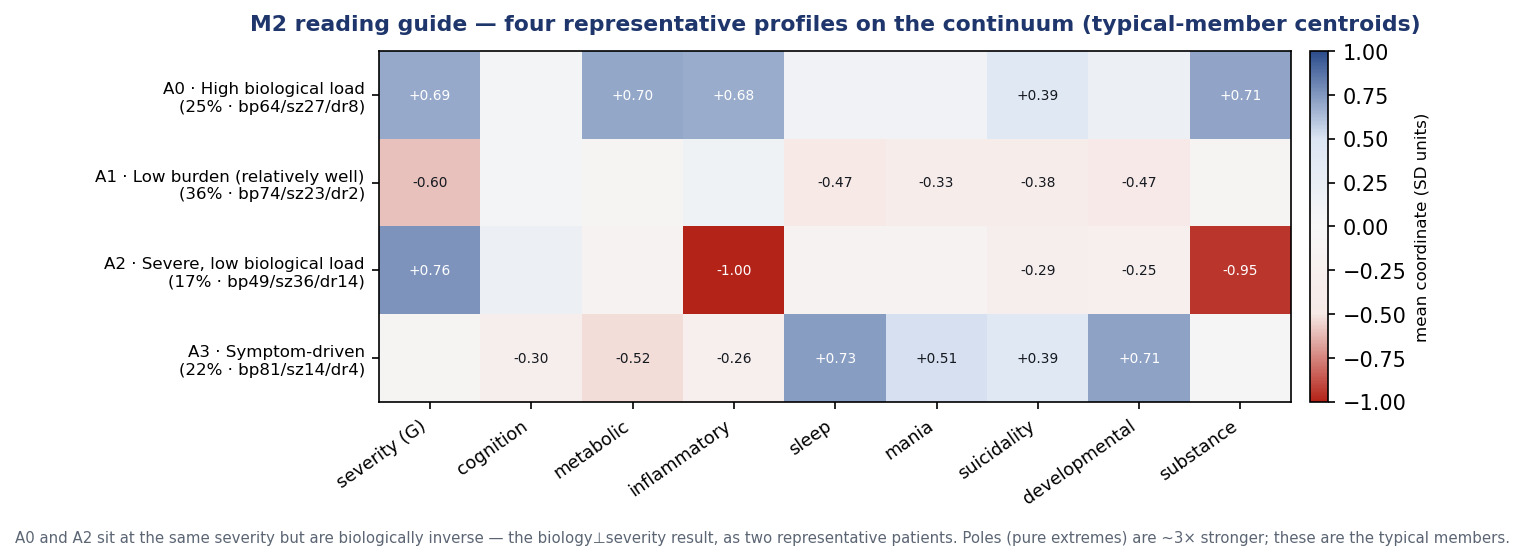
\includegraphics[width=\linewidth]{figures/m2_reading_guide.png}
\caption{The reading guide: four representative profiles (typical-member centroids) on the continuum, plain-
labelled. Red/blue is the mean coordinate per axis (SD units). \textbf{A0} and \textbf{A2} sit at essentially the
\emph{same} severity yet are biologically inverse --- the biology$\perp$severity result, rendered as two
representative patients. Poles (the pure extremes) are $\sim$3$\times$ stronger; these are the typical members.}
\label{fig:readingguide}
\end{figure}

\begin{table}[h]\centering\small\sffamily
\caption{The four corners as a clinical reading guide (Arm A, all nine axes). ``Share'' is the \% of patients
whose dominant pull is this corner; cohort mix is validation-only. Exemplars are cohort-diverse (A2's medoid is a
schizophrenia patient; the rest bipolar) --- the corners are transdiagnostic, not relabelled diagnoses.}
\label{tab:reading}
\begin{tabular}{L{0.5cm} L{3.4cm} R{1.0cm} L{2.6cm} L{5.4cm}}
\toprule
\hdr{} & \hdr{plain label} & \hdr{share} & \hdr{cohorts bp/sz/dr} & \hdr{defining signal}\\
\midrule
\rowcolor{facebg} A0 & High biological load & 25\% & 64 / 27 / 8 & cardiometabolic + inflammatory + substance load, above-average severity\\
A1 & Low burden (well) & 36\% & 74 / 23 / 2 & mild across symptoms and biology\\
\rowcolor{facebg} A2 & Severe, low biology & 17\% & 49 / 36 / 14 & high clinical severity \emph{without} the metabolic/inflammatory/substance signature\\
A3 & Symptom-driven & 22\% & 81 / 14 / 4 & sleep/circadian, early-life adversity, mood activation; near-average severity, low metabolic\\
\bottomrule
\end{tabular}
\end{table}

\begin{keyresult}[The headline, as two patients you can point to]
\textbf{A0 and A2 sit at the same overall severity ($+0.69$ vs $+0.76$) but are biologically opposite}: A0's
representative is high on metabolic/inflammatory/substance ($\approx +0.70$ each), A2's is \emph{low} on all of
them (inflammatory $-1.00$, substance $-0.95$). Two ``typical patients,'' equally ill, biologically inverse ---
the biology$\perp$severity finding made concrete. Crucially, grouping by the corners keeps \textbf{biology the
\emph{defining} axis} of A0's representative; a hard tessellation, by contrast, splits the cloud on suicidality
and shrinks biology to a faint co-loading. This is exactly the heterogeneity a clinician's global impression
cannot see, and what a biology-aware map adds.
\end{keyresult}

\begin{caveatbox}[Corners are a reading lens, not natural kinds]
The four corners describe the \emph{shape} of a continuum; they are not four boxes patients fall into. Most
patients are genuine blends (high corner-entropy; few sit near any pole), and the typical-member centroid is
$\sim$3$\times$ milder than the pure pole --- which is why we report the pole / typical-member / real-exemplar
triplet rather than a single ``type.'' ``A0 vs A2'' is a way to \emph{talk about positions on the map}, not a
claim of discrete kinds.
\end{caveatbox}

\subsection{Reading the map (II): a patient and its nearest neighbours}
\label{sub:similarity}
The most continuum-honest reading needs no corners at all: for any patient, report their position plus their
\textbf{nearest real neighbours} --- the patients most like them. We rank neighbours by an uncertainty-aware
distance so that an axis a patient is poorly measured on does not drive who counts as similar
(Figure~\ref{fig:similarity}).

\begin{methodsbox}[An uncertainty-aware notion of ``similar'']
Each patient is a Gaussian on the map, $\Normal(\mu_i,\,\sigma_i^2)$. We score similarity by
$d^2(i,j)=\sum_d (\mu_{i,d}-\mu_{j,d})^2 / (\sigma_{i,d}^2+\sigma_{j,d}^2)$ --- a per-dimension standardized
distance under the combined measurement uncertainty. A dimension either patient is uncertain about contributes
little, so an ill-measured patient gets a \emph{fuzzy} (less distinct) neighbourhood, exactly as it should. We
compute it two ways: \emph{similar overall} (all nine axes, severity included) and \emph{similar in kind} (the
eight specifics with severity removed --- ``same presentation, regardless of how ill'').
\end{methodsbox}

\begin{figure}[h]\centering
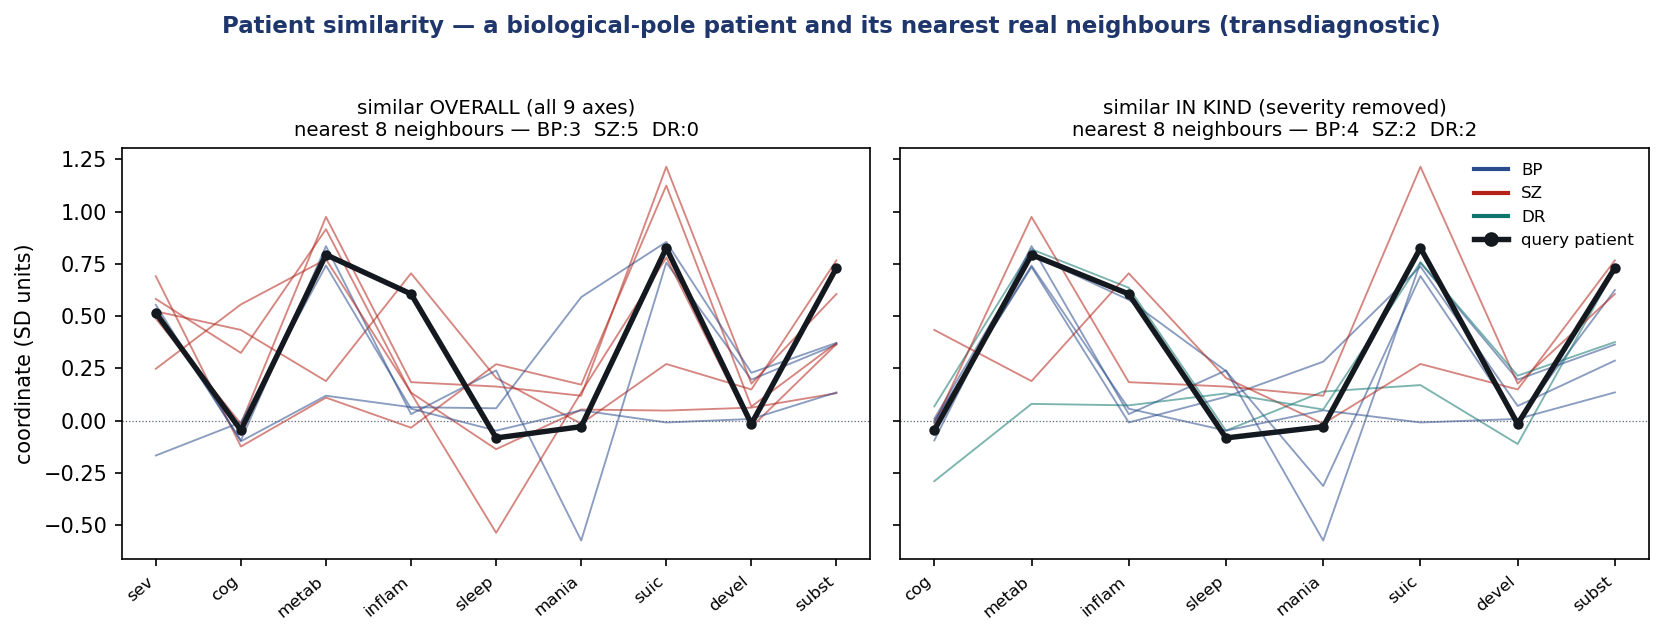
\includegraphics[width=\linewidth]{figures/m2_similarity.png}
\caption{Patient similarity for a biological-pole exemplar (black) and its eight nearest neighbours, coloured by
cohort. \emph{Left:} similar overall. \emph{Right:} similar in kind (severity removed). The neighbours track the
query's profile --- especially its biology --- and are \textbf{transdiagnostic} (a mix of BP/SZ/DR). The two
spaces return different neighbour sets: ``in kind'' frees severity to vary, recovering the phenotype regardless of
how ill the patient is.}
\label{fig:similarity}
\end{figure}

\begin{keyresult}[Transdiagnostic neighbours, and a phenotype that survives severity]
For any patient the tool returns their nearest real neighbours across \emph{all three cohorts} --- the
transdiagnostic promise made operational (``your most similar patients, regardless of diagnosis, look like
this''). And the \emph{in-kind} space recovers clinical kind independent of severity: where the
\emph{overall} neighbours of a symptom-driven patient are a severity-mixed set, the in-kind neighbours are
overwhelmingly other symptom-driven patients (4 of 5 nearest, versus a severity-mixed overall set). Position $+$ neighbours is the continuum-native decision object;
the corners are its human-readable summary.
\end{keyresult}

\subsection{A hard partition, only if you must: the nested $K$-family}
\label{sub:tessellation}
Some workflows need boxes. For them we export a \textbf{nested $K$-family} ($K=2,3,4$) fit by Extreme
Deconvolution (a measurement-error mixture, $x_i\sim\sum_k\pi_k\,\Normal(m_k,V_k+S_i)$, which clusters what
patients \emph{are} after the noise in how they were measured is removed). But we report it as a
\emph{convenience}, not a discovery, for two reasons. First, there is \textbf{no privileged $K$}: the model
evidence is flat across $K$ (XD-BIC $197{,}918$--$198{,}108$, $<0.1\%$). Second, the partition splits the cloud
first on \textbf{suicidality} --- a symptom-burden gradient ($\eta^2$ $0.54$) --- with the biological axes
contributing almost nothing ($\eta^2$ $\approx 0.003$); the specific axes together carry the split
($\eta^2_{\text{specifics}}$ $0.122$) far more than $G$ ($0.008$), but no hard region is ``the biological one.''
A box, in other words, is the wrong tool for the headline. Which $K$ (if any) is operationally useful is an
\emph{outcome} question, deferred to and answered by the prognosis chapter: \emph{none} --- the continuous
position out-predicts every hard partition (\S\ref{sec:prognosis}).

\begin{figure}[h]\centering
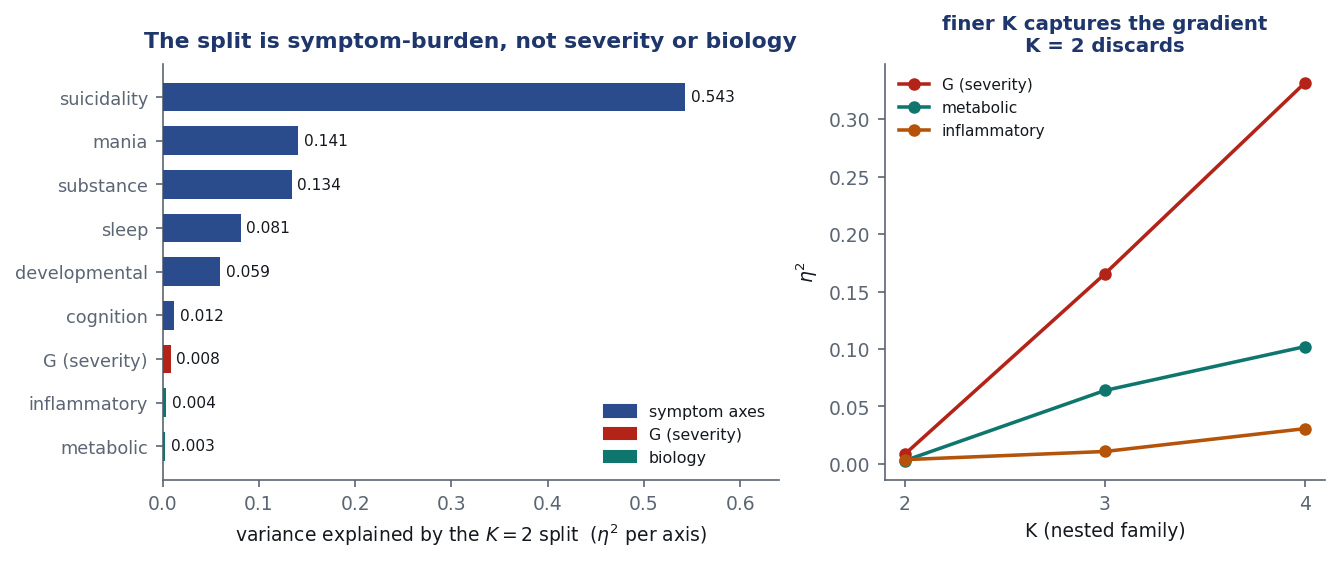
\includegraphics[width=0.96\linewidth]{figures/m2_regions.png}
\caption{The optional $K$-family. \emph{Left:} per-axis variance explained by the $K=2$ split --- it is a
suicidality / symptom-burden gradient, near-blind to biology ($G$ and the biological axes near zero). \emph{Right:}
finer $K$ picks up progressively more of the severity/biology gradient the coarse split discards, but no $K$ is
singled out by the data. A coarse convenience over a continuum, not a set of kinds.}
\label{fig:regions}
\end{figure}

\subsection{Validation: transdiagnostic, stable, not an artefact}
\label{sub:validation}
Whether read as corners or as a coarse partition, the structure passes the checks that matter for using it
(Table~\ref{tab:m2valid}). It is \textbf{transdiagnostic} --- the adjusted Rand index against the three cohorts
and the seven DSM-5 subtypes is $\approx 0$ ($-0.00$ / $0.01$); every corner mixes diagnoses. It is
\textbf{stable} --- re-fits across seeds agree (seed-ARI $0.998$). It is \textbf{not a missingness artefact} --- a
classifier predicting a patient's region from the \emph{pattern of what was measured} scores \emph{below} chance
(coverage permutation $p=0.23$, lift $-0.052$): membership is governed by what patients are, not by who got which
tests. And it is a \textbf{tighter description of the data than diagnosis} --- the free mixture (BIC-best at $K{=}2$) beats a
DSM-5-constrained seven-group one on model evidence (XD-BIC $197{,}963$ vs $201{,}294$), and the coordinates'
variance is four times better explained by the data's own structure than by the diagnostic labels
($\eta^2$ $0.109$ vs $0.025$).

\begin{table}[h]\centering\small\sffamily
\caption{The M2 validation battery (internal/descriptive validity), on the continuous coordinates and the
$K=2$ contract-default partition. The map is transdiagnostic, stable, not a missingness artefact, and a tighter
description than DSM-5.}
\label{tab:m2valid}
\begin{tabular}{L{4.6cm} L{5.6cm} L{3.4cm}}
\toprule
\hdr{question} & \hdr{result} & \hdr{verdict}\\
\midrule
\rowcolor{facebg} Q1 --- does structure exist? & continuum (silhouette $=$ Gaussian null, $z{=}{-}0.36$) & honest: no biotype claim\\
Q2 --- more than severity? & $\eta^2_{\text{specifics}}$ $0.122$ $\gg$ $\eta^2_G$ $0.008$ & specifics drive it\\
\rowcolor{facebg} Q3 --- transdiagnostic? & ARI vs cohort / DSM-5 $=-0.00$ / $0.01$ & cuts across diagnosis\\
Q4 --- stable? & seed-ARI $0.998$ & reproducible\\
\rowcolor{facebg} Q4 --- not an artefact? & coverage$\to$membership perm-$p$ $0.23$, lift $-0.052$ & \textbf{negative} lift\\
vs DSM-5 (BIC) & free $K{=}2$ \textbf{197{,}963} vs DSM-5 7-group $201{,}294$ & tighter, fewer groups\\
\rowcolor{facebg} vs DSM-5 (variance) & coordinate $\eta^2$ \textbf{0.109} vs DSM-5 $0.025$ & DSM-5 barely structures it\\
\bottomrule
\end{tabular}
\end{table}

\begin{figure}[h]\centering
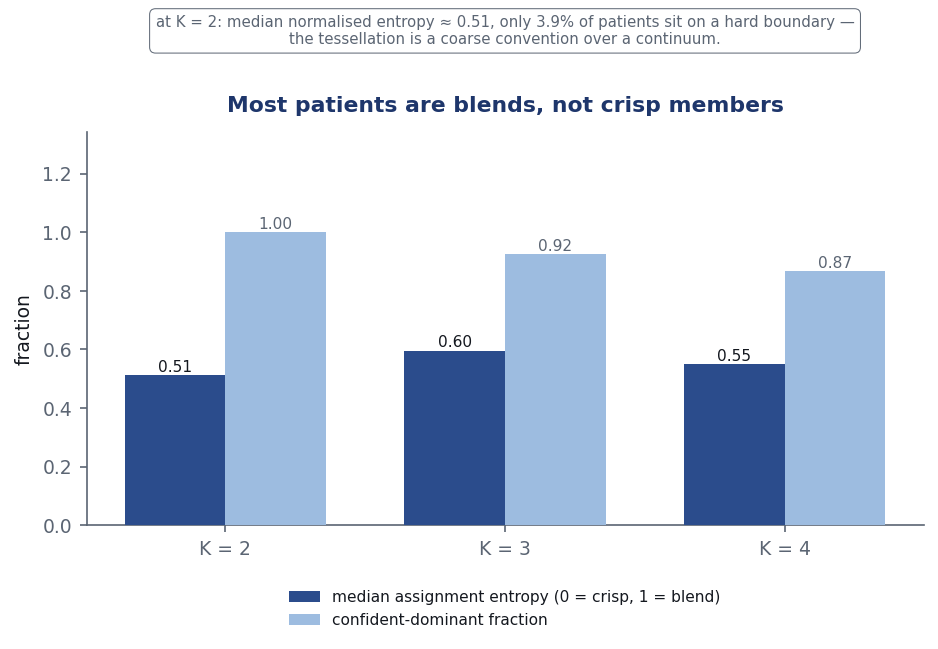
\includegraphics[width=0.86\linewidth]{figures/m2_confidence.png}
\caption{Assignment is soft and honest. Median assignment entropy stays high across the $K$-family and only a few
percent of patients sit on a hard boundary; the archetype simplex is softer still (most patients have no dominant
corner). The softness of the continuum is a reported quantity, never hidden behind a hard label.}
\label{fig:confidence}
\end{figure}

\begin{openbox}[What M2 establishes --- and what it defers]
M2 converts the map into a usable, continuum-honest object: a \textbf{validated transdiagnostic coordinate
system}, with a \textbf{reading guide} (four representative profiles, biology$\perp$severity made pointable) and a
\textbf{patient-similarity} tool (transdiagnostic nearest neighbours). It establishes, under internal/descriptive
validity, that this structure is real, stable, transdiagnostic, specific-axis-driven, not a missingness artefact,
and tighter than the diagnostic labels --- and that it is a \emph{continuum}, so the corners and the optional
$K$-family are reading lenses, not natural kinds. What it does \emph{not} yet claim is any predictive, prognostic,
temporal, or treatment value. The decisive tests come next: \textbf{temporal coherence} (do the coordinates
persist? \S\ref{sec:temporal}), \textbf{prognosis} (do they predict beyond diagnosis $+$ severity, and which
granularity earns its keep? \S\ref{sec:prognosis}), and \textbf{treatment} (do they moderate response?
\S\ref{sec:treatment}).
\end{openbox}
